\chapter{Convex Learning Problems}

Another potential, and common way to limit the hypothesis space is to assert that it is convex. The following group of exercises will be concerned with this assertion.

\begin{definition}[Convex set]
	A set $ C $ is said to be \defined{convex} if for every pair of points $ a,b \in C $, the following inclusion holds,
	\begin{align*}
		\{ \lambda a + (1- \lambda) b: \lambda \in [ 0,1 ] \} \subseteq C
	\end{align*}
\end{definition}

There is a good geometric intuition for this definition. In particular, the set which must be included in $ C $ describes the straight line from $ a $ to $ b $. So, a set $ C $ is convex if and only if it contains every straight line between any two points. See the figure below.

\begin{figure}[!htb]
	\centering
	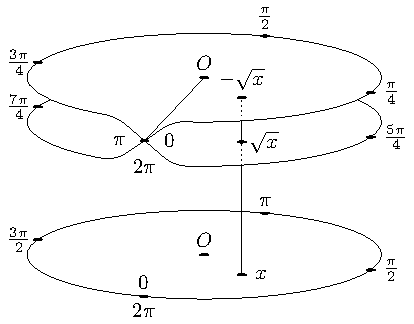
\includegraphics{convex-sets/figure.pdf}
	\caption{The set $ C $ is convex, but since we can find a line which is not contained in the set $ N $, this set is not convex.}
\end{figure}

